\section{CI/CD}

\subsection{Choice of a CI/CD system}

Since our project is hosted in a GitHub repository, the most natural choice for our CI/CD system was GitHub Actions. It is also the de facto standard in the industry, with the skills learned being transferable to other CI/CD systems.

\subsection{Pipeline}
Workflows are located in \texttt{.github/workflows/}. The main pipeline, \texttt{ci.yml}, runs on every push and pull request targeting \texttt{main}. The first four jobs run in parallel, the fifth (\texttt{uitest}) job depends on them all completing. All five must pass before the \texttt{deploy} job runs:

\begin{enumerate}
    \item \texttt{gofmt}: uses \texttt{gofumpt} to check whether every Go file in the repo follows its formatting rules
    \item \texttt{golangci}: runs the \texttt{golangci-lint} linter on the Go code to check for bugs, style problems, and common mistakes
    \item \texttt{hadolint}: \texttt{Dockerfile} linter
    \item \texttt{integration\_test}: runs Go integration tests that make HTTP requests to verify the endpoints work correctly
    \item \texttt{uitest}: runs Selenium UI tests to verify that the user interface works as intended
    \item \texttt{deploy}: deploys to production, but only after all previous jobs pass
    \item \texttt{codeql}: runs GitHub's CodeQL static analyzer on the Go code to check for security vulnerabilities
    \item \texttt{image\_scan}: builds the production container image and runs Trivy on it to check for fixable HIGH/CRITICAL vulnerabilities in OS packages and Go dependencies
\end{enumerate}

The pipeline flow and diagram can be seen in figure \ref{fig:ci_pipeline}.
\begin{figure}
    \centering
    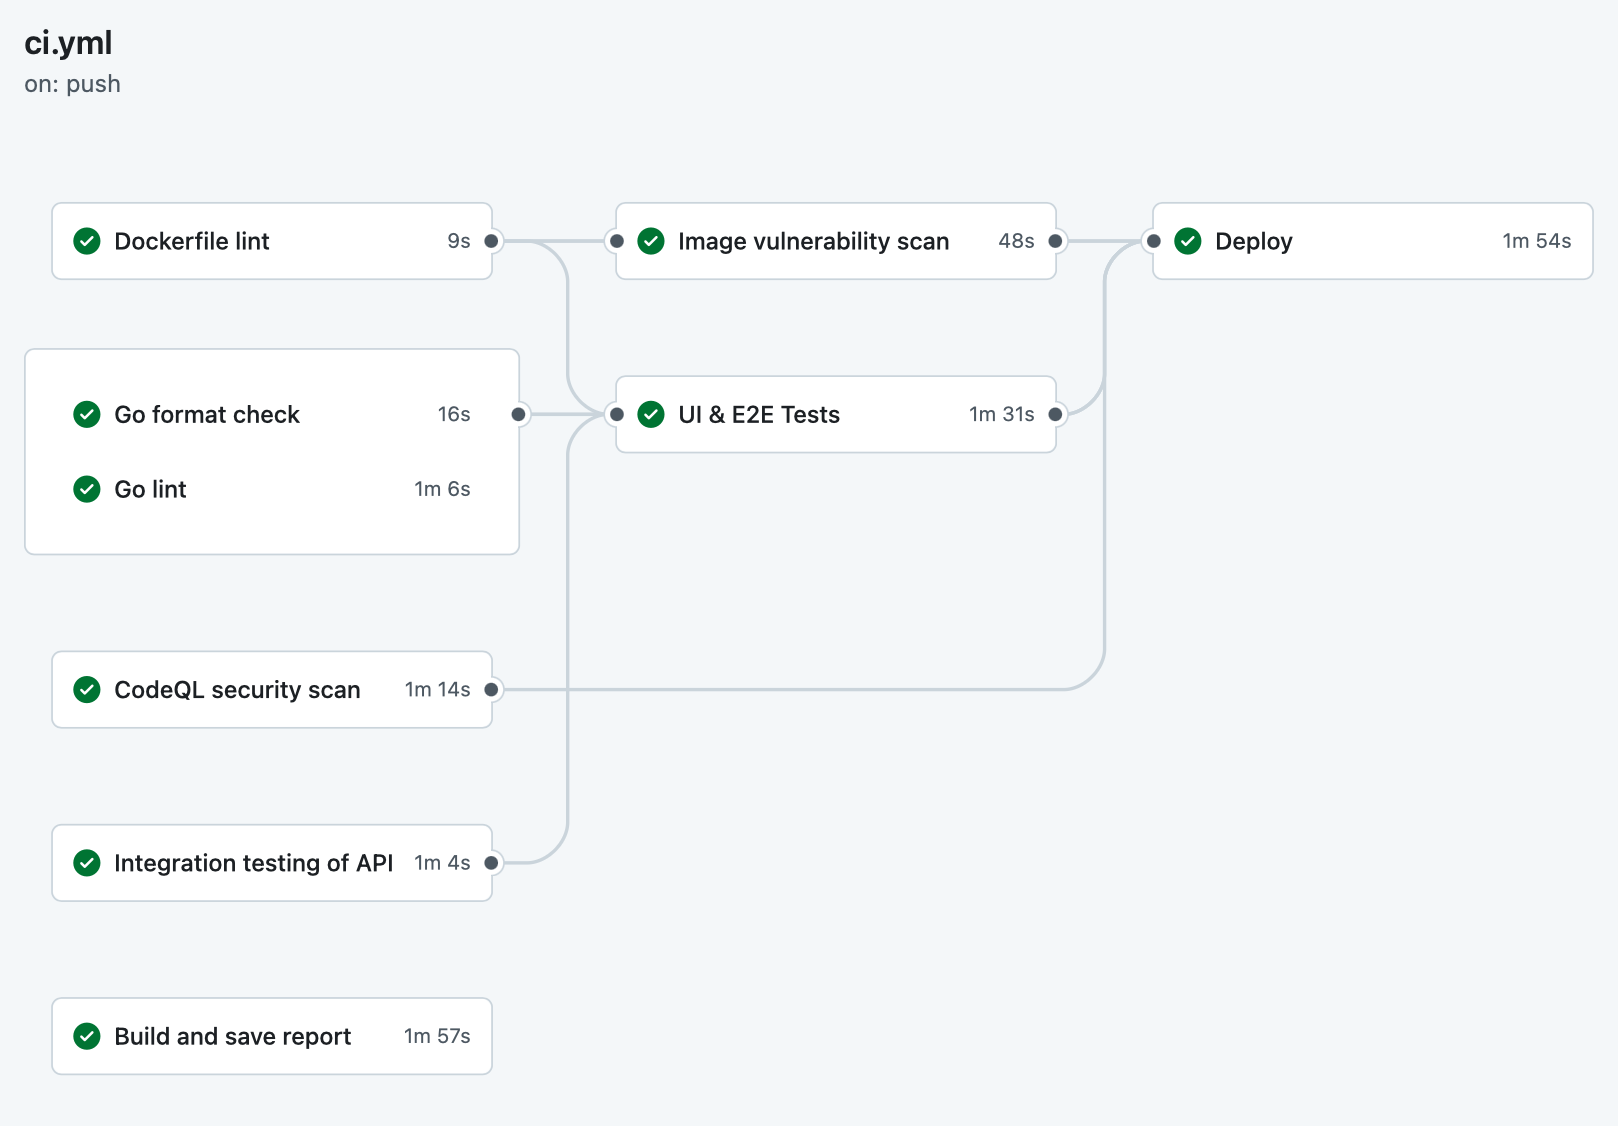
\includegraphics[width=0.8\linewidth]{report/images/cicd.png}
    \caption{CI/CD pipeline flow diagram}
    \label{fig:ci_pipeline}
\end{figure}

The \texttt{deploy} job additionally requires \texttt{github.ref == \texttt{refs/heads/main}} -- meaning that pull requests run the full pipeline but only merges into main actually deploy.

\subsection{Deployment}
The deploy job SSH-es into the server as a dedicated \texttt{deploy} user using a private key stored in GitHub Secrets. The \texttt{deploy} user is a member of the \texttt{docker} group, which allows the user to run docker containers without \texttt{sudo} privileges.  The \texttt{deploy} user then loads environment variables from \texttt{.env}, pulls the latest \texttt{main}, builds the Docker image, deploys the stack using \texttt{docker-compose.yml}, and updates the web service with the new image.

\subsection{Releases}
We use a \texttt{weekly-release.yml} workflow that runs every Friday at 9:00 UTC, and creates a GitHub Release tagged \texttt{release-YYYY-MM-DD} with auto-generated release notes with every merged pull request since the previous release tag.